% ============================================================
%  Chapter fragment -- included by main.tex
%  (not a standalone document; compile main.tex to build the PDF)
% ============================================================

\sheettitle{06 -- PenTesting 3: Threat Modeling $\to$ Post-Exploitation}{SWS2 -- ZHAW / Tellenbach}

Covers PTES phases \kw{3 Threat Modeling}, \kw{4 Vuln Analysis}, \kw{5 Exploitation}, \kw{6 Post-Exploitation} + the \kw{Metasploit} framework.

% ==================== THREAT MODELING ====================
\section{Threat Modeling (Phase 3)}

\subsection{Attacker- vs Defender-centric \hl{(!)}}
\begin{itemize}
\item \kw{Attacker-centric} (\kw{building} SW, SWS1): "\kw{list every threat} to this design $\to$ so we know what to defend." Identify threats $\to$ find design vulns $\to$ derive new \kw{security requirements}. \kw{Broad \& systematic}, throughout the \kw{SDLC}. Methods: \kw{STRIDE}, \kw{Attack Trees}.
\item \kw{Defender-centric (offensive)}: "given these \kw{existing defenses}, find the \kw{best route around them} to the asset." \kw{Targeted} -- most promising path from \kw{attack surface} to \kw{targeted assets} (pentester simulating a real threat actor).
\end{itemize}
\textit{Ex: building a login} -- attacker-centric asks "how abused?" $\to$ \kw{password spraying / brute force} $\to$ add control (rate-limit / lockout / MFA). That control \kw{is the output}. Later, \kw{defender-centric} = the pentester sees the lockout+WAF and asks "best way \kw{past} it?" (spray slowly under the limit, or pivot to an endpoint without the protection). \hl{Attacker-centric builds the defense; defender-centric probes a path past it.}

\subsection{Attack surface}
"The set of ways an adversary can \kw{enter the system} \& cause damage." Built from \kw{intelligence-gathering} data. Attacker uses the system's \kw{entry \& exit points} (interfaces) -- \kw{exit points} give the attacker \kw{feedback}. Relevant points depend on \kw{attacker model} + \kw{scope} (e.g. OSSTMM channels).

\subsection{Pentester workflow}
\begin{enumerate}
\item Understand the org's \kw{defenders} \& where they fortified.
\item \kw{Process-flow diagrams}: map attack surface $\to$ assets along \kw{multiple paths}.
\item Map \kw{defensive capabilities} as check-points/mitigations \kw{to avoid}.
\item Identify \& \kw{prioritize useful targets} + attack vectors.
\end{enumerate}
\textit{A process-flow diagram annotates components with \kw{Assets} (A01..), \kw{Controls} (C01..) \& \kw{Threat Agents} (TA01..).}

\begin{center}
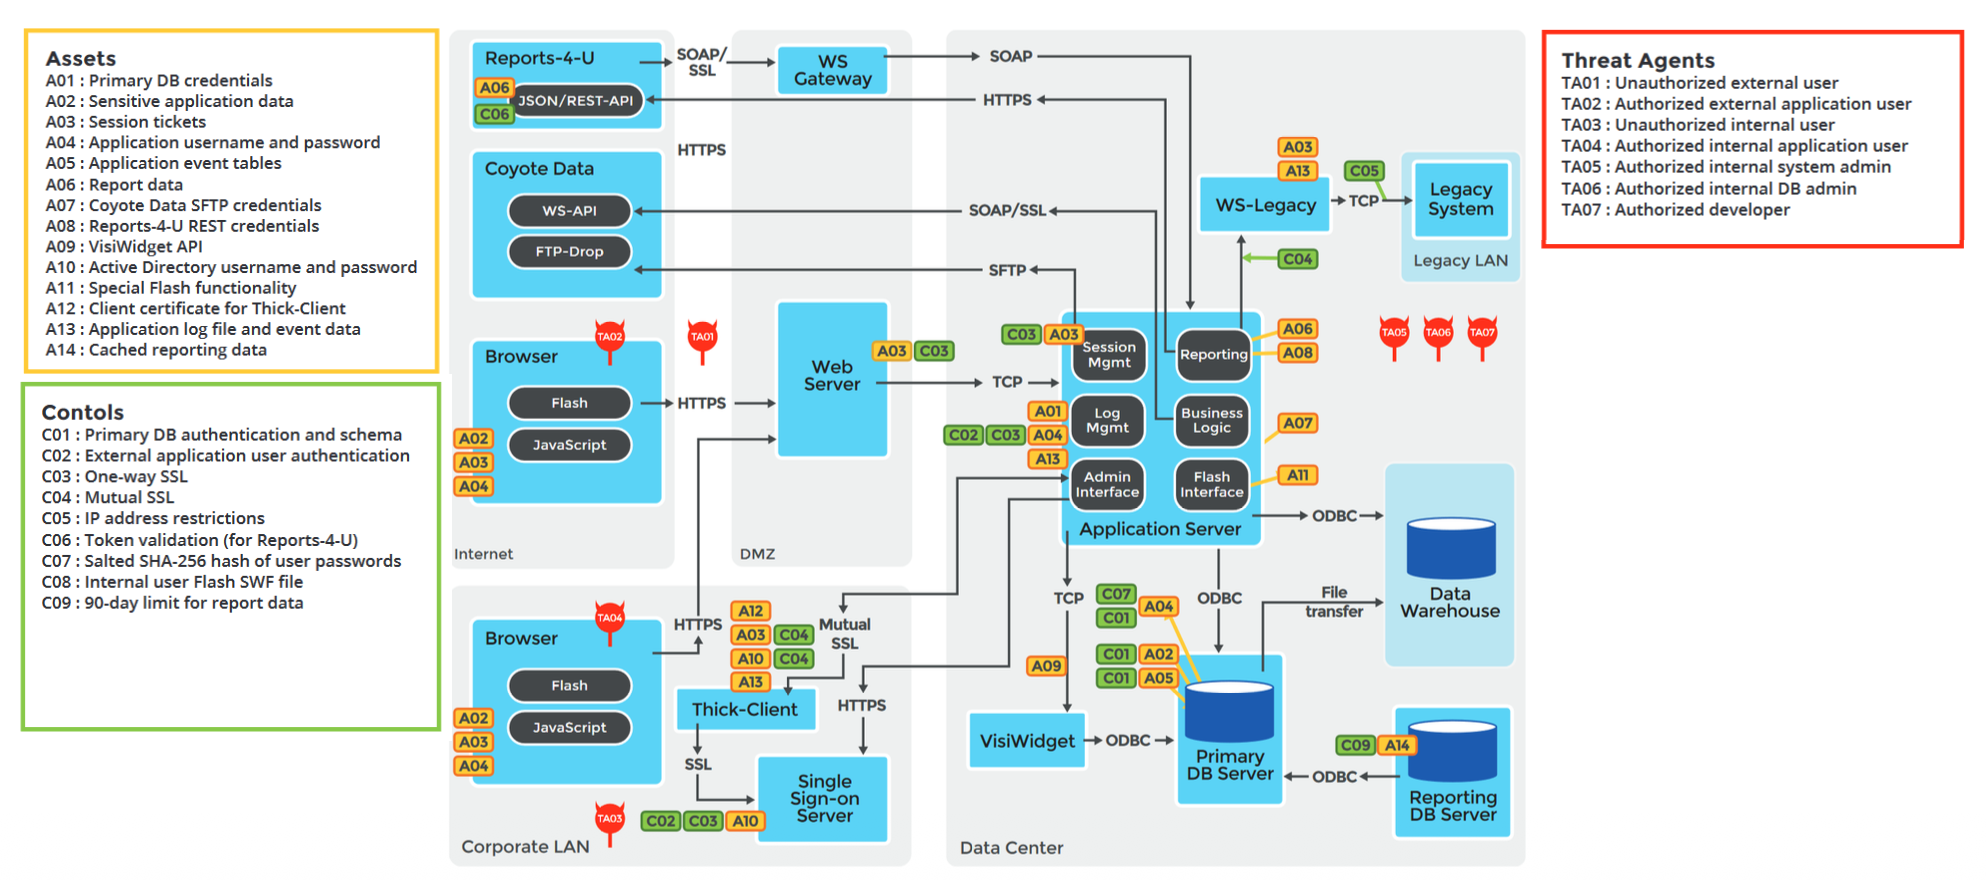
\includegraphics[width=\linewidth]{Figures/process_flow_diagram_pentesting.png}
\end{center}


\subsection{Primary \& Secondary Assets \hl{(!)}}
\begin{itemize}
\item \kw{Primary asset}: part of the system \kw{under test (in scope)}.
\item \kw{Secondary asset}: \kw{not in scope} but shared with / linked to in-scope assets.
\item Primary compromise can \kw{imply} secondary compromise. Secondary assets change \kw{which threat agents} matter.
\end{itemize}
\textit{Ex (CRM pentest):} primary = customer DB + CRM webserver. Secondary = \kw{HR employee DB on the same DB server}. With primary only, \kw{insiders irrelevant} (staff already have CRM access); considering secondary, \kw{insiders become relevant} (salaries/health data) $\to$ CRM is a \kw{stepping stone} to employee data.

\subsection{Attack Patterns: MITRE \hl{(!)}}
Organize knowledge about \kw{adversary behavior} (key for red-teaming):
\begin{itemize}
\item \kw{CAPEC} (Common Attack Pattern Enumeration \& Classification): focus \kw{application security}; enumerates \kw{exploits} vs vulnerable systems; incl. social-eng/supply-chain; linked to \kw{CWE} (weaknesses). Organized by \kw{Mechanisms} (1000) \& \kw{Domains} (3000: SW/HW/Comms/Supply Chain/Social Eng/Physical).
\item \kw{ATT\&CK} (Adversarial Tactics, Techniques \& Common Knowledge): focus \kw{network defense}; from threat-intel + red-team; \kw{contextual} understanding of malicious behavior; the \kw{Enterprise Matrix} (tactics as columns: Recon $\to$ ... $\to$ Impact).
\end{itemize}
\textbf{Use \kw{CAPEC}} for: app threat modeling, dev training, \kw{pentesting}. \textbf{Use \kw{ATT\&CK}} for: comparing CND capabilities, \kw{defending vs APT}, threat hunting, \kw{adversary emulation}. They are \kw{cross-referenced}.
\textit{A CAPEC entry gives: description, attack \kw{execution flow}, related \kw{CVE}s, probing techniques, attacker \kw{skill} required, consequences, mitigations.}

% ==================== VULNERABILITY ANALYSIS ====================
\section{Vulnerability Analysis (Phase 4)}
\kw{Discover \& confirm} security issues (misconfig $\to$ insecure design). Process \kw{depends on the component} (web app, network, building, employees).
\textbf{Goals:} validate vulns \kw{exist} (as \kw{employee} w/ creds, as \kw{outsider} w/o, with/without mitigations); or validate a \kw{mitigation works} (= not exploitable).

\subsection{Discovery methods}
\begin{itemize}
\item \kw{Port scanners}: e.g. an answer on TCP 23 (telnet) might itself be a vuln.
\item \kw{Well-known-vuln scanners}: \kw{product+version} $\to$ lookup in vuln DB; or \kw{recipe/signature}-based (run a script, e.g. test a known buffer overflow, weak TLS, default passwords).
\item \kw{New vulns}: type-specific (\kw{sqlmap} = SQLi, \kw{XSStrike} = XSS), \kw{web-app} scanners (crawl/user-supplied URLs), \kw{source-code} scanners (custom SW), \kw{manual} code/system analysis (e.g. \kw{CIS Benchmark} hardening guides).
\end{itemize}

\subsection{Generic-scanner recipe}
1) Determine all \kw{reachable assets} (IPs, ports, domains -- nmap, sublist3r). 2) Determine \kw{products/technologies} (nmap, BuiltWith/Wappalyzer for web). 3) \kw{Match} known-vuln DBs vs identified products+versions. 4) Run product-specific recipes/scanners. \textit{Proprietary (Nessus) = own engine; \kw{meta-scanners} (scanmeter.io) merge several open-source scanners.}

\subsection{Challenges -- FP / FN \hl{(!)}}
\begin{itemize}
\item \kw{When to scan?} new vuln data added continuously.
\item \kw{Product+version is misleading}: forked/renamed product $\to$ \hl{false negative}; \kw{patched without version bump} (\kw{backporting}, e.g. RedHat) $\to$ \hl{false positive}.
\item Results depend on \kw{time/location/account}: intranet vs extranet (filters between), \kw{authenticated vs unauthenticated}.
\end{itemize}

\subsection{Active analysis: fuzzing}
\kw{Fuzzers} find \kw{unknown} vulns (black-box vs advanced; ideally test \kw{offline}; app/protocol-specific, e.g. X.509/SOAP). \term{Ex: American Fuzzy Lop (AFL)} -- compile-time \kw{instrumentation} + \kw{genetic algorithms} to find inputs that \kw{trigger new internal states}.

\subsection{Tracking}
Track what's been analysed (esp. teams). \kw{Attack trees} document extensive tests with many patterns; \kw{evolve} as new systems found; avoid \kw{repeating} work when attack vectors "merge".

\subsection{Vuln Scanner: Nessus}
\begin{itemize}
\item Most popular \kw{generic} scanner (OS $\to$ server $\to$ web app "layers"); commercial (Tenable), free non-commercial \kw{$\leq$16 IPs}.
\item Tests = \kw{plugins} in \kw{NASL} (Nessus Attack Scripting Lang.); \kw{GVM / OpenVAS} (Greenbone) is a \kw{fork}, also NASL. GVM free = \kw{community feed only} (lacks many enterprise products).
\item Runs via \kw{daemons} (usually intranet; Internet scan complements). Place daemons w.r.t. firewalls; beware \kw{alarms} in your own detective controls.
\item Config: IP ranges, plugins, \kw{auth-scan} creds; disable \kw{Safe Checks} to run \kw{unsafe} plugins (ACT\_DESTRUCTIVE, ACT\_DENIAL, ACT\_KILL\_HOST, ACT\_FLOOD).
\end{itemize}
\textit{Ex results (FP vs TP):}
\begin{itemize}
\item \kw{"SSL Cert Cannot Be Trusted"} = Medium. Means the cert's \kw{chain of trust} doesn't reach a \kw{known public root CA} -- here because it's signed by a \kw{private/own CA} (issuer = "Marc Rennhard Private CA"), not DigiCert/Let's Encrypt/etc. (self-signed = same idea, signs itself). $\to$ \hl{false positive}: \kw{intentional} for an internal service (the right clients have that private CA root installed, so they \kw{do} trust it). Scanner only sees "not chained to a public root". Would be a \kw{true positive} on a \kw{public-facing} site (real browsers warn $\to$ MitM opening).
\item \kw{Weak 40-bit ciphers} = \hl{true positive}, Medium reasonable (not easily exploitable).
\end{itemize}
\hl{Point:} scanner flags on a \kw{technical rule}; whether it's a real problem needs \kw{context it lacks} $\to$ human verification.

% ==================== EXPLOITATION ====================
\section{Exploitation (Phase 5)}
Focus solely on \kw{establishing access} by \kw{bypassing security restrictions}. An \kw{exploit} = software / chunk of data / command sequence that \kw{takes advantage of a vuln} (gain control, extract/manipulate data, priv-esc, DoS).

\subsection{Precision Strike \hl{(!)}}
Each attack vector is assessed by \kw{P(success)} \& \kw{P(detected)} (from threat-modeling + vuln-analysis). Choose the \kw{most promising} vector $\to$ hit precisely, minimize noise.

\subsection{Attack vectors}
Web-app (XSS+cookie, SQLi) \textbullet{} \kw{memory-based} (buffer/heap overflow, use-after-free) \textbullet{} MitM \textbullet{} USB drop \textbullet{} password cracking / breaking crypto \textbullet{} hardware (DMA) \textbullet{} \kw{social engineering} if nothing else works. \textit{Value of a pentest = \kw{creativity} + precise exploitation.}

\subsection{Challenges \& circumvention}
\begin{itemize}
\item Develop exploits where \kw{none exists yet} (e.g. for fuzzing finds).
\item Security controls interfere: AV, \kw{app whitelisting}, IPS, WAF, \kw{DEP}, \kw{ASLR}, \kw{stack canaries}.
\item Circumvention (hard): \kw{encode/pack/encrypt} payload, keep it \kw{memory-resident}; whitelisting $\to$ \kw{process injection} / in-memory malware; DEP/ASLR/canaries $\to$ exploitation-lab techniques.
\end{itemize}

\subsection{Level of expertise}
\begin{itemize}
\item \kw{White belt}: use public exploits via frameworks; known social-eng.
\item \kw{Green belt}: test/modify public exploits (evasion); tune frameworks; tailored social-eng.
\item \kw{Black belt}: \kw{zero-day} -- reverse-engineer/fuzz/analyse to find \& exploit \kw{undiscovered} vulns; reproduce target env incl. countermeasures.
\end{itemize}

% ==================== POST EXPLOITATION ====================
\section{Post-Exploitation (Phase 6)}
You're now \kw{inside} a machine. Two jobs:
\begin{itemize}
\item \kw{Determine the value} of what you compromised -- how \kw{sensitive} is its data, and how useful is it for \kw{breaking in further}?
\item \kw{Maintain control} of it for later use.
\end{itemize}

\hl{Most dangerous phase} -- the tester sits on the client's \kw{real, critical systems} where a mistake could \kw{cause harm} (delete data, crash production). $\Rightarrow$ the \kw{RoE} (\kw{Rules of Engagement} -- the pre-agreed contract on \kw{how} testing may happen: what's allowed, when, how evidence is handled) is what \kw{keeps day-to-day operations \& data safe} here.

\subsection{Pivoting / island hopping / lateral movement}
All three names = the \kw{same idea}: once you own \kw{host A}, use \kw{A as a launch pad} to attack \kw{host B} deeper in the network.
\begin{itemize}
\item Why it works: from \kw{inside}, A is a \kw{trusted insider} -- it can reach machines a firewall would \kw{block from the outside}.
\item \term{Ex:} you can't hit the internal DB from the Internet, but the web server you popped \kw{can} $\to$ attack the DB \kw{through} the web server.
\item In Metasploit: \kw{route add <subnet> <session>} routes your tools \kw{through} the compromised host (see Meterpreter).
\end{itemize}

\subsection{Maintaining access}
\hl{Careful with backdoors} -- \kw{someone else might connect} to your "service". To persist \& evade: known remote-mgmt tools, built-in tools, \kw{custom fileless backdoors}, obfuscation/morphing. \textit{Fileless: macros / scripts (PowerShell, WMI, BITSAdmin) / registry \& task-scheduler persistence.}

% ==================== METASPLOIT ====================
\section{Metasploit Framework (MSF) \hl{(!)}}
Open-source platform (\kw{Ruby}) to \kw{develop, test \& use} exploit code; interoperates with port/vuln scanners. \kw{Free} (web GUI dropped 2019) vs \kw{Pro} (GUI, automation, reporting, \kw{IDS/AV evasion}). \textit{Others: Exploit Pack, Core Impact, IMMUNITY CANVAS.}

\subsection{msfconsole}
All-in-one console (\kw{msfconsole -q} = no banner); readline/tab-completion; can run external commands. Key cmds: \kw{search}, \kw{use}, \kw{show options/info}, \kw{set/setg}, \kw{sessions}.

\subsection{Architecture}
\begin{itemize}
\item \kw{Rex}: sockets, protocols, text transforms (SSL, SMB, HTTP, Base64...).
\item \kw{MSF::Core}: basic API (Datastore, ModuleManager, Session Manager...).
\item \kw{MSF::Base}: simplified APIs. \kw{MSF::UI}: Console/CLI/WebUI/GUI.
\item \kw{Penetration Modules} = "the meat" (see below).
\end{itemize}

\begin{center}
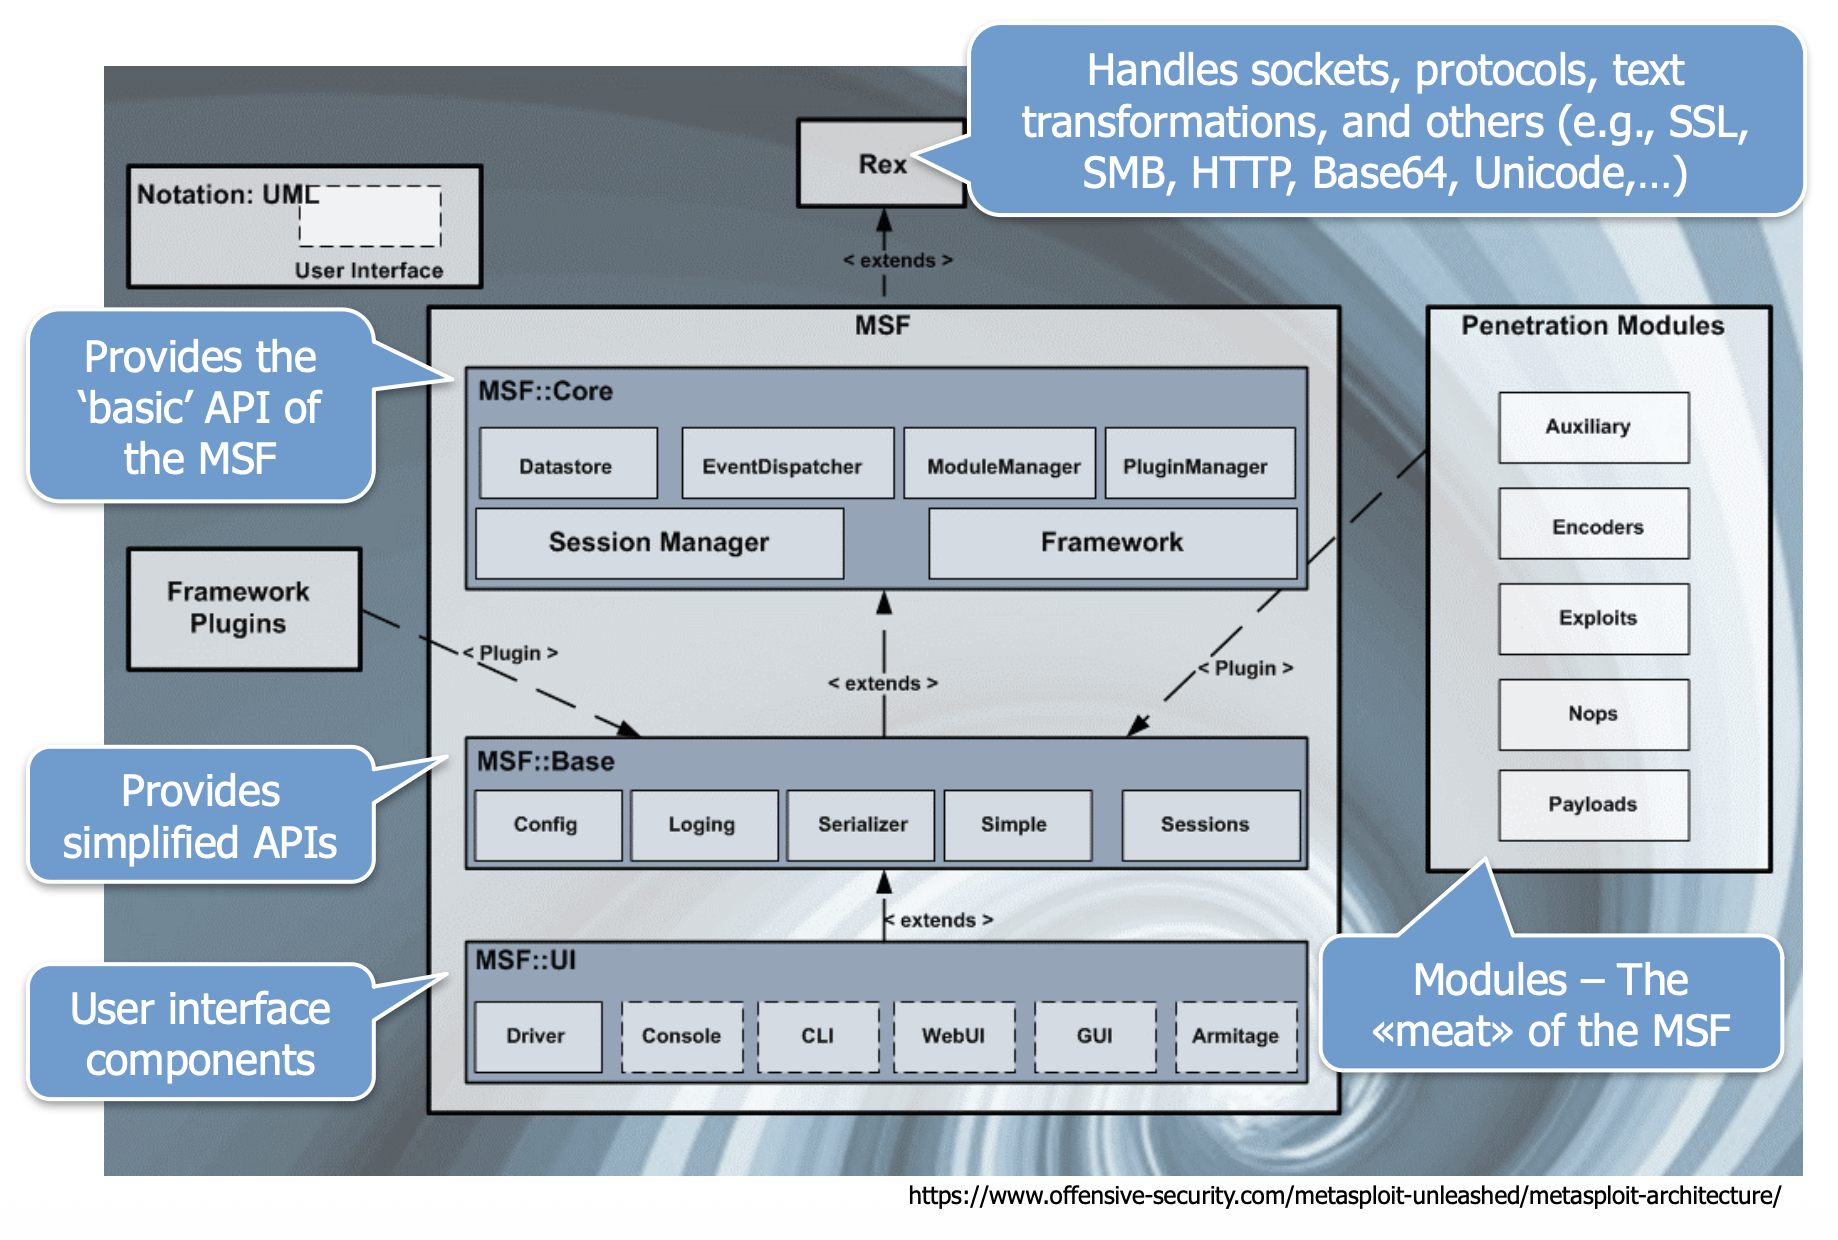
\includegraphics[width=\linewidth]{Figures/metasploit_architecture.png}
\end{center}

\subsection{Module types}
All modules = Ruby classes. (\kw{/usr/share/metasploit-framework/modules/}, custom in \kw{$\sim$/.msf4/modules/}.)
\begin{itemize}
\item \kw{Exploits}: exploit a vuln + place/run a payload. (Exploit w/o payload, e.g. DoS-only $\to$ \kw{Auxiliary}.)
\item \kw{Auxiliary}: port scanners, fuzzers, sniffers, brute-forcers, DoS.
\item \kw{Payloads}: the code that runs on the target.
\item \kw{Encoders}: ensure payloads \kw{reach} the target (evade/encode). \kw{Nops}: keep payload size consistent.
\end{itemize}

\subsection{Exploits: active vs passive}
\begin{itemize}
\item \kw{Active}: exploit a \kw{specific host}, run to completion \& exit (\kw{-j} = background).
\item \kw{Passive}: \kw{wait for incoming} connections from client software (browsers \& others); shells created in background (\kw{-l} list sessions, \kw{-i} interact).
\end{itemize}
\textit{Usage:} \kw{use <exploit>} $\to$ \kw{show options} (set RHOSTS/RPORT...) $\to$ pick payload $\to$ \kw{show options} (set LHOST/LPORT) $\to$ run.

\subsection{Payloads \hl{(!)}}
\begin{itemize}
\item \kw{Singles}: \kw{self-contained} (fire-and-forget); victim need not connect back; can be \kw{big} (needs vuln allowing many bytes). E.g. add user / run calc.exe.
\item \kw{Stagers}: set up a \kw{network connection} attacker$\leftrightarrow$victim to fetch more; \kw{small} (for vulns allowing few bytes).
\item \kw{Stages}: components \kw{downloaded by stagers} (e.g. \kw{Meterpreter}, VNC injection).
\end{itemize}
Generate standalone: \kw{use <payload>} $\to$ \kw{generate -f exe -o mlwr.exe}.

\subsection{Meterpreter}
Advanced \kw{post-exploitation} payload via \kw{library (DLL) injection}; \kw{stealthy} = \kw{in-memory}, no disk access, no new process. Can: run commands, \kw{in-memory process migration}, registry/filesystem, API scripting, \kw{pivoting \& port forwarding}.
\textit{Cmds:} \kw{upload}/\kw{execute} files; \kw{route add 192.168.2.0 255.255.255.0 <sid>} = route through a session into the victim's internal net (pivoting).

\subsection{Post-exploitation modules}
\kw{gather} (data/enumeration) \textbullet{} \kw{gather/credentials} \textbullet{} \kw{gather/forensics} \textbullet{} \kw{manage} (migration/injection) \textbullet{} \kw{recon} (no stealing) \textbullet{} \kw{escalate} (priv-esc) \textbullet{} \kw{wlan} \textbullet{} \kw{capture} (keylogging).

\begin{defbox}
\textbf{Take-away:} Threat modeling, vuln analysis, exploitation \& post-exploitation involve many skills. \kw{Vuln scanners aren't perfect} -- legit \kw{false positives} (backported patch) \& \kw{false negatives} (renamed product). \kw{Metasploit} makes exploiting well-known vulns easy.
\end{defbox}

